\documentclass{article}[10pt]
\usepackage{amsmath}
\usepackage{amssymb}
\usepackage{amsthm}
\usepackage{booktabs}
\usepackage{float}
\usepackage{graphicx}
\usepackage[margin=1in]{geometry}
\usepackage{pgfplots}
\usepackage[utf8]{inputenc}
\usepackage{siunitx}
\usepackage{subcaption}
\usepackage{tikz}
\usepackage{wrapfig}

\graphicspath{ {Images/} }
\pgfplotsset{width=8cm,compat=1.14}
\usetikzlibrary{backgrounds,shadows,fit,positioning}


\begin{document}
\section{Wave-particle duality}
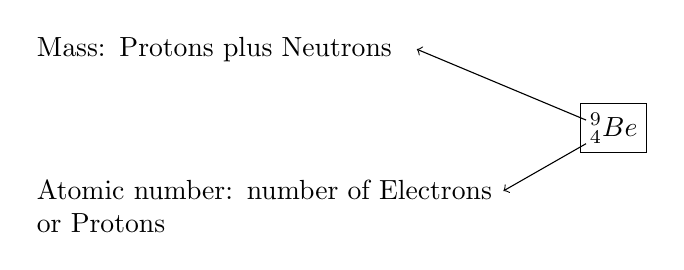
\begin{tikzpicture}
	\draw (0.2,0) node {$\boxed{{}^9_4Be}$};
	\draw [left, text width=6cm](-1,1) node {Mass: Protons plus Neutrons};
	\draw [left, text width=6cm](-1,-1) node {Atomic number: number of Electrons or Protons};
	\draw [->] (-0.15,-0.2) -- (-1.2,-0.8);
	\draw [->] (-0.15,0.1) -- (-2.3,1);
\end{tikzpicture}

\subsection{Characteristics of a Wave}
\begin{itemize}
	\item Wave Length ($\lambda$) --- Distance between two consecutive points of
	      equal vibrational phase.
	      \begin{center}
	      	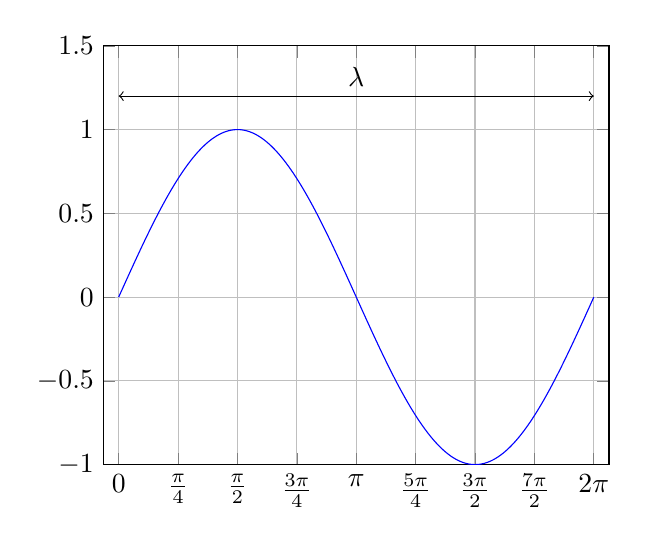
\begin{tikzpicture}
	      		\begin{axis}
	      			[
	      			domain=0:2*pi,
	      			samples=200,
	      			xmin=-0.2,
	      			xmax=2*pi+0.2,
	      			ymin=-1,
	      			no marks,grid,
	      			xticklabels={0, $\frac{\pi}{4}$,  $\frac{\pi}{2}$,
	      				$\frac{3\pi}{4}$, $\pi$,$\frac{5\pi}{4}$,
	      				$\frac{3\pi}{2}$, $\frac{7\pi}{2}$, 2$\pi$},
	      			xtick={0, 0.7853,...,6.2832},
	      			ymax=1.5
	      			]
	      			\addplot {sin(deg(x))};
	      			\draw[<->]      (0,1.2) -- node[above] {$\lambda$} (6.2832,1.2);
	      		\end{axis}
	      	\end{tikzpicture}
	      \end{center}
	      \begin{align*}
	      	1\si{\micro\metre} = \num{e-6}\si{\metre} \\[0.5em]
	      	1\si{\nano\metre} = \num{e-9}\si{\metre}  \\[0.5em]
	      	1\si{\angstrom} = \num{e-10}\si{\metre}   \\[0.5em]
	      	1\si{\pico\metre} = \num{e-12}\si{\metre} \\[0.5em]
	      \end{align*}
	\item Frequency ($\nu$) --- Number of vibrations or complete cycles per
	      unit of time.
	      \begin{align*}
	      	1\si{\mega\hertz} = \num{e6}\si{\hertz}  \\[0.5em]
	      	1\si{\giga\hertz} = \num{e9}\si{\hertz}  \\[0.5em]
	      	1\si{\tera\hertz} = \num{e12}\si{\hertz} \\[0.5em]
	      \end{align*}

	\item Period ($T$) --- Duration of a cycle $V=\frac{1}{T}$

	\item Wavenumber --- Number of complete cycles per unit of time
	      \begin{align*}
	      	\bar{\nu} = \frac{1}{\lambda}
	      \end{align*}
	\item Propagation Speed --- Speed with which the wave propagates in a given
	      direction.
	      \begin{align*}
	      	\nu = \frac{c}{\lambda} \\
	      	\lambda = cT
	      \end{align*}
	      \begin{center}
	      	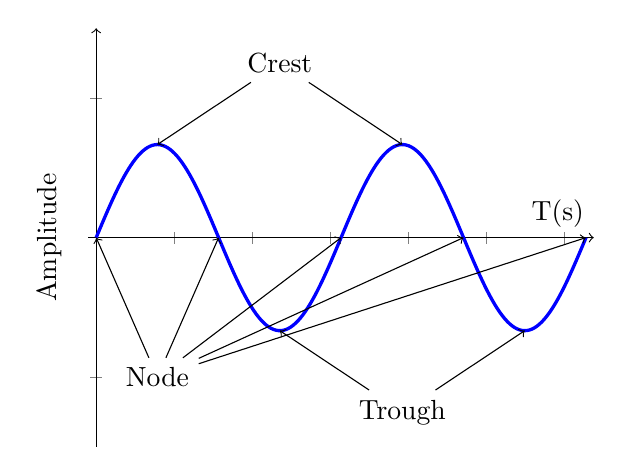
\begin{tikzpicture}
	      		\begin{axis}
	      			[
	      			axis lines=middle,
	      			axis line style={->},
	      			xmin=-0.2,
	      			xmax=4*pi+0.2,
	      			xticklabels={,,},
	      			xlabel={T($\si{\second}$)},
	      			ymin=-1.5,
	      			ymax=1.5,
	      			yticklabels={,,},
	      			ylabel={Amplitude},
	      			ylabel near ticks,
	      			]
	      			\addplot[blue, very thick,samples=200,domain=0:4*pi] {(sin(deg(x)))/1.5};
	      			\node (crest) at (1.5*pi, 1.25) {Crest};
	      			\node (trough) at (2.5*pi, -1.25) {Trough};
	      			\node (node) at (0.5*pi, -1) {Node};
	      			\draw[->] (crest) -- (0.5*pi, 1/1.5);
	      			\draw[->] (crest) -- (2.5*pi, 1/1.5);
	      			\draw[->] (trough) -- (1.5*pi, -1/1.5);
	      			\draw[->] (trough) -- (3.5*pi, -1/1.5);
	      			\draw[->] (node) -- (0,0);
	      			\draw[->] (node) -- (pi,0);
	      			\draw[->] (node) -- (2*pi,0);
	      			\draw[->] (node) -- (3*pi,0);
	      			\draw[->] (node) -- (4*pi,0);
	      		\end{axis}
	      	\end{tikzpicture}
	      \end{center}

\end{itemize}
Note that the frequency, and the period are, unlike the wavelegth, independent
of the mean through which the wave travels.
\subsection{Energy of an Electromagnetic Wave}
\begin{align*}
	E & = h\nu &   & E=nh\nu \\
\end{align*}
Where $E$ is the energy of a photon or electron, $h$ is Planck's constant
($h = 6.62607\times 10^{-34}\si{\joule\second}$)
\subsection{Electromagnetic Spectrum}
TODO:\@ Figure out how to sensibly align/display these
\begin{figure}[H]
	\centering
	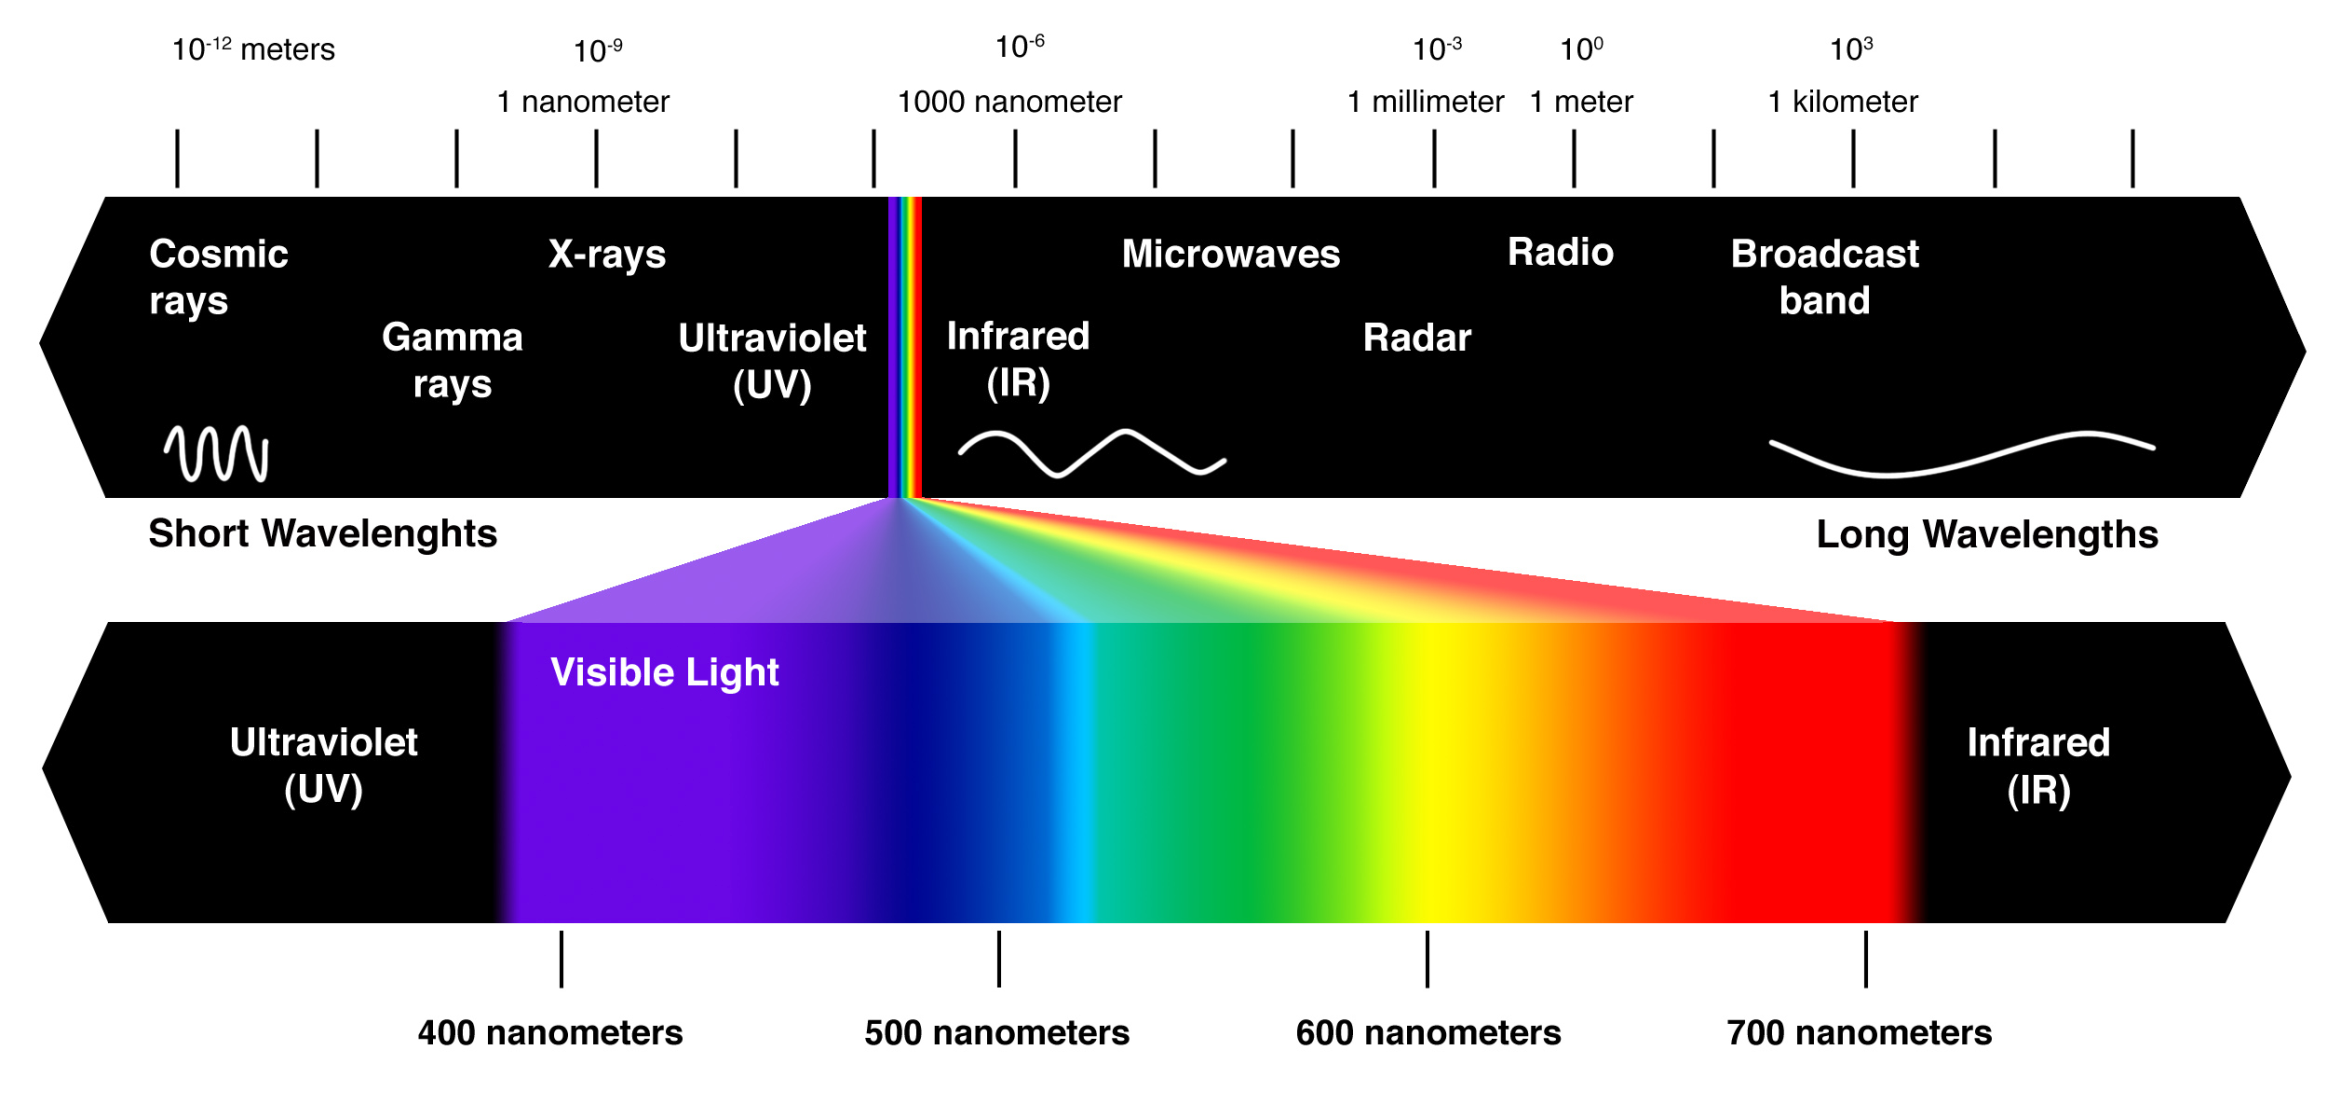
\includegraphics[scale=0.6]{radiations}
\end{figure}
\begin{figure}
	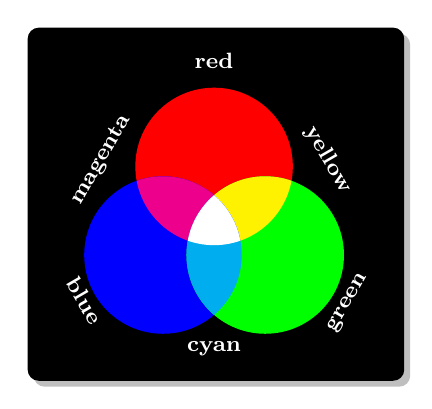
\begin{tikzpicture}[line width=0]
		\foreach \angle/\col in {90/red,210/blue,330/green}{
			\fill[fill=\col] (\angle:.75) circle (1cm);
		}
		\foreach \angle/\col in {90/yellow,210/magenta,330/cyan}{
			\begin{scope}
				\clip (\angle:.75) circle(1cm);
				\fill[fill=\col] (\angle-120:.75) circle (1cm);
			\end{scope}
		}
		\begin{scope}
			\clip (90:.75) circle(1cm);
			\clip (210:.75) circle(1cm);
			\fill[fill=white] (330:.75) circle (1cm);
		\end{scope}
		\foreach \name/\angle/\dist\reta in {%
			red/90/2/0, yellow/30/1.6/0,%
			green/-30/2/180, cyan/-90/1.6/180,%
			blue/-150/2/180, magenta/150/1.6/0%
			} {%
			\node[rotate=\angle-90+\reta,anchor=base,minimum width=3.8em,
			font=\bfseries\footnotesize,text=white] at (\angle:\dist)
			{\name};%
		}
		\begin{pgfonlayer}{background}
			\node(cadre)[drop shadow,fit=(current bounding box),rounded corners,
			line width=1pt,fill=black,inner sep=2mm]{};
		\end{pgfonlayer}
	\end{tikzpicture}
	\caption{Light Interferences}
\end{figure}
\subsection{Interference}
Interference is a phenomenom associated with the wave-like behavior of
electromagnetic radiation. The interference between two waves travelling through
the same region in space yields another wave, which is the algebric sum of the
two interferring waves.
\begin{figure}[H]
	\pgfplotsset{
		axis lines=middle,
		axis line style={->},
		xmin=0,
		xmax=4.2*pi,
		xticklabels=empty,
		xtick=\empty,
		ymin=-1,
		ymax=1,
		yticklabels=empty,
		ytick=\empty,
		samples=200,
		domain=0:4*pi,
		every axis plot post/.append style={very thick},
		clip=false
	}% end of common axis set

	\begin{subfigure}[b]{0.4\textwidth}
		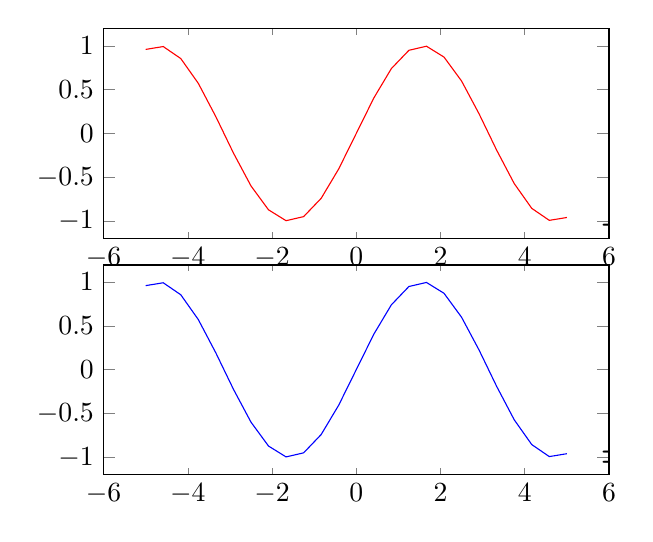
\begin{tikzpicture}
			\begin{axis}% 1. plot
				[yscale=0.5]
				\addplot[red] {(sin(deg(x)))};
				\node at (2*pi,-1.05) {\huge$+$};
			\end{axis}
			\begin{axis}% 2. plot
				[ yshift=-3cm, yscale=0.5]
				\addplot[blue] {(sin(deg(x)))};
				\node at (2*pi,-1.05) {\huge$=$};
			\end{axis}
		\end{tikzpicture}

		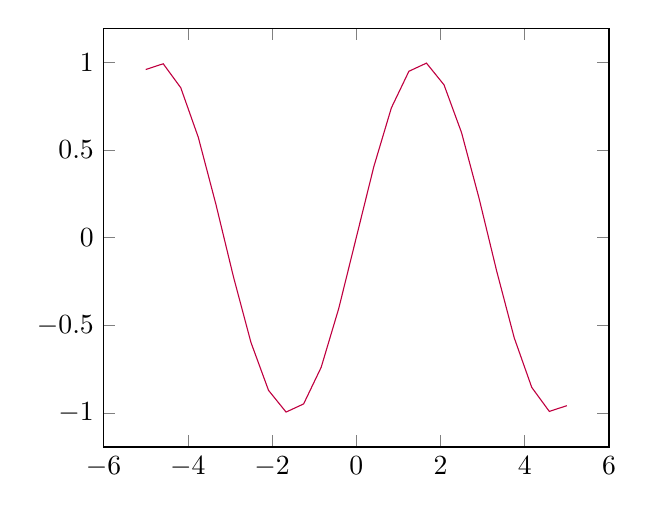
\begin{tikzpicture}
			\begin{axis}% 3. plot
				\addplot[purple] {(sin(deg(x)))};
			\end{axis}
		\end{tikzpicture}
		\caption{Constructive interference}
	\end{subfigure}
	\hfill %%%% %%%% %%%% second image
	\begin{subfigure}[b]{0.4\textwidth}
		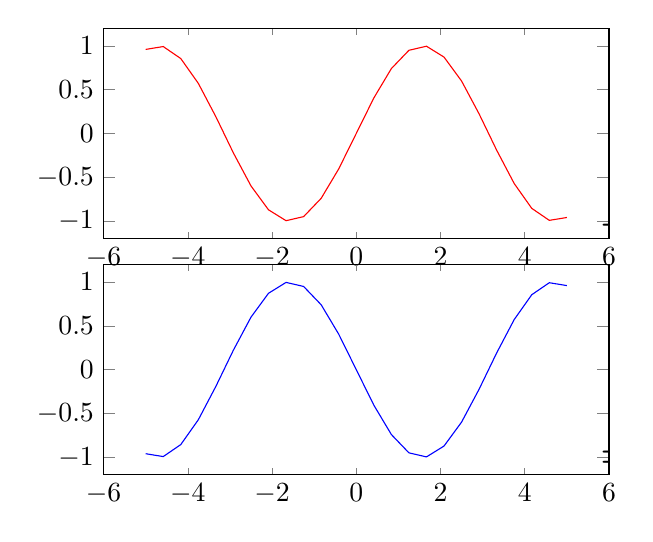
\begin{tikzpicture}
			\begin{axis}% 1. plot
				[yscale=0.5]
				\addplot[red] {(sin(deg(x)))};
				\node at (2*pi,-1.05) {\huge$+$};
			\end{axis}
			\begin{axis}% 2. plot
				[ yshift=-3cm,yscale=0.5]
				\addplot[blue] {(sin(deg(x+pi)))};
				\node at (2*pi,-1.05) {\huge$=$};
			\end{axis}
		\end{tikzpicture}

		\begin{tikzpicture}
			\begin{axis}% 3. plot
				\addplot[purple] {0};
			\end{axis}
		\end{tikzpicture}
		\caption{Destructive interference}
	\end{subfigure}
\end{figure}

\subsection{Stationary Waves}
REVIEW NEEDED

The interference between two waves travelling at the same speed, but in opposing
directions creates a \emph{stationary wave} --- a wave in which, throughout
time, the nodes, crests, ans troughs stay at the same point in space.

The existence of boundary conditions, beyond causing the phenomenon to be
stationary, has another important consequence.The wave functions that describe
it [the wave] cannot be ordinary. It's wavelength depends on imposed physical
constraints (in this case a distance between points in space) and differ
from each other through an integer.
\[
	\lambda = \frac{2L}{n} \qquad n=1,2,3,\ldots \\
\]

With this we can see that the solutions are discrete, as opposed to being continuous, and the
factor distinguishing them is the integer $n$, which we call a quatum number.
\begin{figure}[H]
	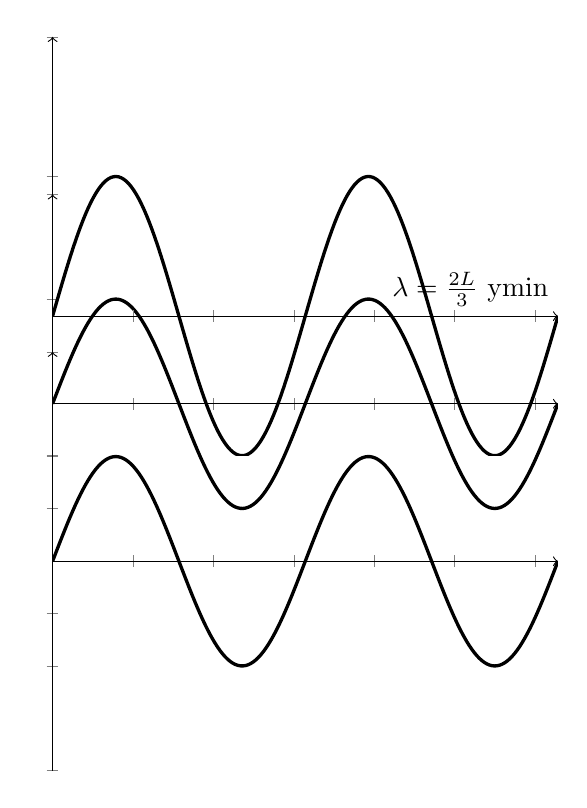
\begin{tikzpicture}
		\begin{axis}
			[
			axis lines=middle,
			axis line style={->},
			xmin=0,
			xmax=4*pi,
			xticklabels={,,},
			ymin=-1,
			ymax=1,
			yticklabels={,,},
			]
			\addplot[black, very thick,samples=200,domain=0:4*pi] {(sin(deg(x))/2)};
		\end{axis}
		\begin{axis}
			[
			yshift=2cm,
			axis lines=middle,
			axis line style={->},
			xmin=-0,
			xmax=4*pi,
			xticklabels={,,},
			xlabel={$\lambda = \frac{2L}{3}$}
			ymin=-1,
			ymax=1,
			yticklabels={,,},
			]
			\addplot[black, very thick,samples=200,domain=0:4*pi] {(sin(deg(x))/2)};
		\end{axis}
		\begin{axis}
			[
			yshift=-2cm,
			axis lines=middle,
			axis line style={->},
			xmin=-0,
			xmax=4*pi,
			xticklabels={,,},
			ymin=-1,
			ymax=1,
			yticklabels={,,},
			]
			\addplot[black, very thick,samples=200,domain=0:4*pi] {(sin(deg(x))/2)};
		\end{axis}
	\end{tikzpicture}
\end{figure}

TODO:\@ Fix this. No idea how to make it work as intended.
\subsection{Electromagnetic Radiation}
The propagation of electromagnetic radiation is a wave-like movement, and with
it we associate a period $T$, a frequency $\nu$, and a wavelength $\lambda$.
While in some cases the eletromagnetic radiation will present typical wave-like
behavior, such as diffraction, on others it behaves in  a particle-like manner.
One example of the particle-like nature of radiation is the well known
``photoelectric effect'' experiment.

TODO:\@ Diagram of the photoelectric setup.

From this experiment we could verify that:
\begin{enumerate}
	\item The emission of electrons on off the plate depends on the frequency of
	      the incident radiation, and not on the intensity of the inciding beam.
	\item The number of emitted electrons is proportional to the intensity of
	      the beam
	\item Emission is imediate, even for low-intensity beams.
	\item Electrons bind (connect) to the metal with an energy $W$, which has to
	      the incident beam must provide to release the electron. The kinetic
	      energy of said electron is such that:
	      \begin{align*}
	      	E_c & = \frac{1}{2}\si{\metre\newton}^2 = E_{\text{photon}} - W \\
	      	E_c & = h\nu - W                                                \\
	      \end{align*}
\end{enumerate}
Below a certain \emph{critical frequency} $\nu_0$, there will be no
photoemission, because the energy $h\nu$ is insufficient to ``beat''
the attraction potential $W$. We then have
$$h\nu_0 = W$$
TODO:\@ Add the graph that is at the beginning of page 5.

The intensity of the inciding beam will be a measurement of the number of
\emph{quanta} transmitted by the radiation, given that the higher the intensity
the more photons are emitted per unit of time. The interpretation of the
photoelectric effect suggests that light is a particle, and that the energy for
each transmitted particle is $h\nu$. Einstein named these particles \emph{photons}.

In other experiments, such as the dark-body emission, the particle-like
description of light is the only one compatible with the results. We can now see
that the wave-like and particle-like aspects of light are intimately associated,
and that the best description of radiation is a \emph{dual} one.
\subsection{de-Broglie Hypothesis}
\begin{align*}
	E=h\nu                            & \qquad E=mc^2                      \\
	h\nu=mc^2 \iff h\frac{c}{\lambda} & = mc^2 \iff \lambda = \frac{h}{mc} \\
\end{align*}
Analogally, for a particle moving at speed other than $c$ we have $\lambda = \frac{h}{mv}$

de-Broglie, with the dualistic properties of radiation in mind,
proposed that this type of behavior, verified for electromagnetic radiation,
would be valid for all the other entities which had, up until that point, been
identified as particles. He would later describe this idea with the
relation:
$$\lambda = \frac{h}{p}$$
\subsection{Electrons}
\begin{itemize}
	\item Particle-like Behavior
	      \begin{itemize}
	      	\item The determination of the mass of the electron attributed to
	      	      it a particle-like characteristic.
	      \end{itemize}
	\item Wave-like Behavior
	      \begin{itemize}
	      	\item Electrons suffer difraction when interferring with crystals.
	      \end{itemize}
\end{itemize}
\subsection{Heisenberg's Uncertainty Principle}
A direct consequence of the dualistic behavior is the impossibily of measuring
with precision the position and the momentum of a particle. Subsequently we
must, at the quantum level, abandon the concept of trajectory since, to describe
it we must know at any given time the position and momentum of a given particle.
\subsection{Schrödinger's Equation}
\begin{figure}[H]
	\centering
	\begin{align*}
		E = E_p + E_k \iff E\psi = (E_p + E_k)\psi                                   \\
		\iff -\frac{h^2}{8\pi^2 m}\frac{d^2\psi(x)}{dx^2} + E_p\psi(x) = E_{\psi(x)}
	\end{align*}
	\caption*{Time independent Schrödinger equation on 1 dimension, describing any system that exibits particle-wave behavior}
\end{figure}

Where $\psi$ is the wave function.
\subsection{Physical Interpretation of Schrödinger's solutions}

The wave function $\psi(x)$ does not have any physical meaning at first, but
it's square $\psi{(x)}^2$ is proportional to the density of particles at the point
$x$.

If $\psi(x)$ represents a single particle, it's square will be \emph{probability density}
of finding said particle at a point $x$.

\subsection{Particle in a Box}
Imagine a particle (electron, photon, and so on) confined to a region in space,
unidimensional and of length $a$. It is limited (confined) by two ``walls'' of
infinite potential, or an energy well.

TODO:\@ Get the 0 to show on the x axis label.
TODO:\@ Align this to the right.
\begin{figure}[H]
	\begin{tikzpicture}
		\begin{axis}
			[
			axis lines=middle,
			xticklabels={,,},
			ymin=0,
			ymax=10,
			yticklabels={,,},
			ylabel={$V(x)$},
			xtick={0,1,...,10},
			xticklabels={0,,,,,,,,,,$a$},
			xmin=0,
			xmax=10,
			xlabel={$x$},
			]
		\end{axis}
		\begin{axis}
			[
			xshift=0cm,
			axis lines=middle,
			xtick={0,-1,...,-10},
			xticklabels={,,},
			ymin=0,
			ymax=10,
			yticklabels={,,},
			xmin=-10,
			xmax=0,
			]
		\end{axis}
	\end{tikzpicture}
	\caption{Energy well. $\forall x\le 0 \vee x\ge a : E_p=\infty$, also $\forall 0<x<a : E_p=0 $}
\end{figure}
\begin{equation*}
	E_n=\frac{n^2h^2}{8mL^2}
\end{equation*}
The index $n$ on the energy is marking that the different possible energy levels
for the system depend only on an integer $n$. Conversely, the varying wave
functions depend only on the quantum number $n$.
\begin{equation*}
	\psi_n(x) = \sqrt{\frac{2}{L}}\sin{\frac{n\pi x}{L}}
\end{equation*}
We now have a set of tuples $(\psi_n(x), E_n)$ which are solutions to
Schrödinger's equation, when applied to a particle of mass $m$ constrained in an
energy well.
TODO:\@ The following graphics are kind of a mess. Fix them.
\begin{figure*}

	\begin{subfigure}[b]{0.5\textwidth}
		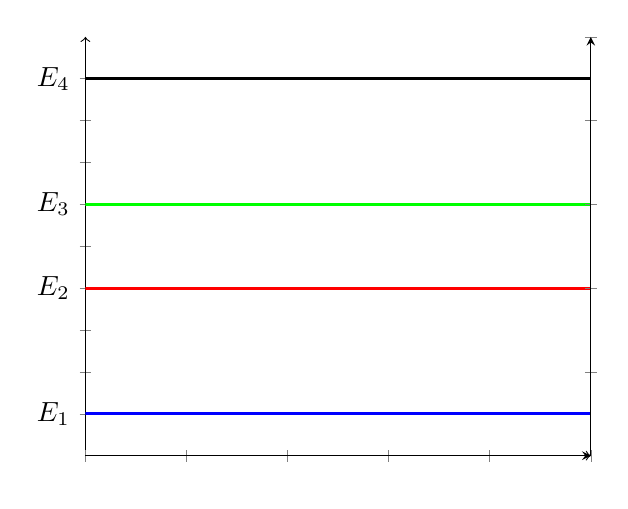
\begin{tikzpicture}
			\begin{axis}
				[
				axis lines=middle,
				axis line style={->},
				xmin=0,
				xmax=5,
				xticklabels={,,},
				ymin=0,
				ymax=10,
				ytick={0,1,...,9},
				yticklabels={,$E_1$,,,$E_2$,,$E_3$,,,$E_4$},
				ylabel near ticks,
				]
				\addplot[blue, very thick,samples=200,domain=0:5] {1};
				\addplot[red, very thick,samples=200,domain=0:5] {4};
				\addplot[green, very thick,samples=200,domain=0:5] {6};
				\addplot[black, very thick,samples=200,domain=0:5] {9};
			\end{axis}
			\begin{axis}
				[
				xshift=0cm,
				axis lines=middle,
				xticklabels={,,},
				ymin=0,
				ymax=10,
				yticklabels={,,},
				xmin=-5,
				xmax=0,
				]
			\end{axis}
		\end{tikzpicture}
		\caption{Three first energy levels allowed for a particle in a potential box}
	\end{subfigure}
	\begin{subfigure}[b]{0.5\textwidth}
		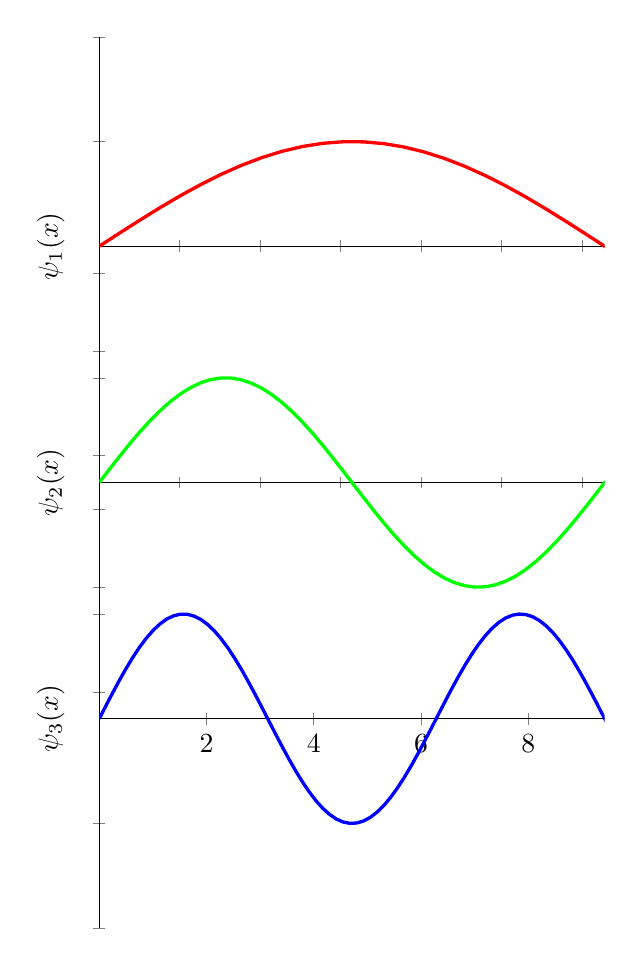
\begin{tikzpicture}
			\begin{axis}
				[
				axis lines=middle,
				axis line style={-},
				ymin=-1, ymax=1,
				xmin=0, xmax = pi,
				ylabel={$\psi_1(x)$},
				ytick={-1,-0.5,...,0.5,1},
				yticklabels={,,},
				xticklabels={,,},
				ylabel near ticks,
				]
				\addplot[red, very thick,samples=200,domain=0:8*pi] {(sin(deg(x+pi))/2)*-1};
			\end{axis}
			\begin{axis}
				[
				yshift=-3cm,
				axis lines=middle,
				axis line style={-},
				ymin=-1, ymax=1,
				xmin=0, xmax = 2*pi,
				ylabel={$\psi_2(x)$},
				ytick={-1,-0.5,...,0.5,1},
				yticklabels={,,},
				xticklabels={,,},
				ylabel near ticks,
				]
				\addplot[green, very thick,samples=200,domain=0:8*pi] {(sin(deg(x+pi))/2)*-1};
			\end{axis}
			\begin{axis}
				[
				yshift=-6cm,
				axis lines=middle,
				axis line style={-},
				ymin=-1, ymax=1,
				xmin=0, xmax = 3*pi,
				ylabel={$\psi_3(x)$},
				ytick={-1,-0.5,...,0.5,1},
				yticklabels={,,},
				ylabel near ticks,
				]
				\addplot[blue, very thick,samples=200,domain=0:8*pi] {(sin(deg(x+pi))/2)*-1};
			\end{axis}
		\end{tikzpicture}
		\caption{Three first wave functions for a given system}
	\end{subfigure}
	\newline
	\begin{center}
		\begin{subfigure}[b]{0.5\textwidth}
			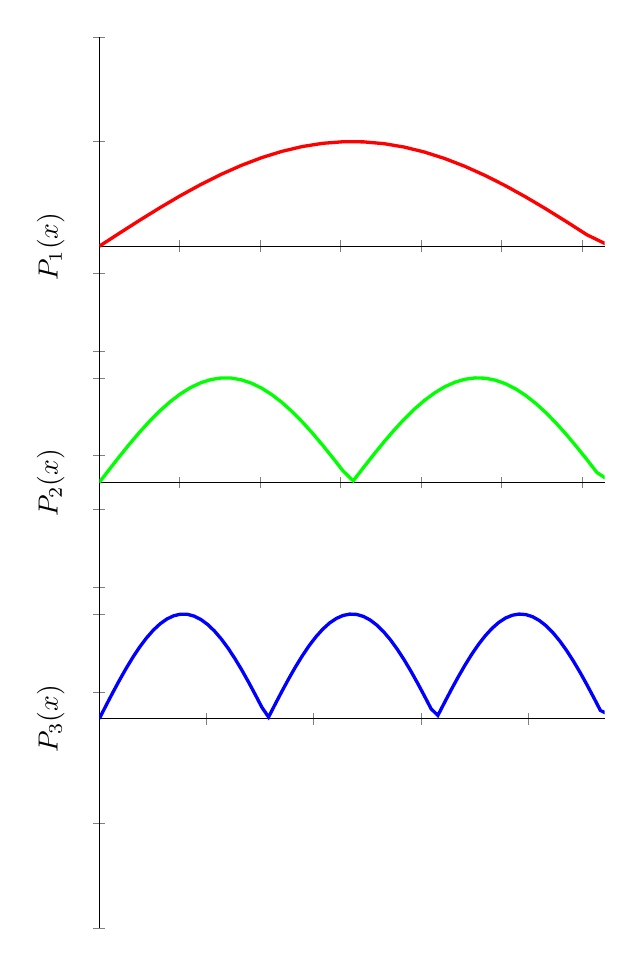
\begin{tikzpicture}
				\begin{axis}
					[
					axis lines=middle,
					axis line style={-},
					ymin=-1, ymax=1,
					xmin=0, xmax = pi,
					ylabel={$P_1(x)$},
					ytick={-1,-0.5,...,0.5,1},
					yticklabels={,,},
					xticklabels={,,},
					ylabel near ticks,
					]
					\addplot[red, very thick,samples=200,domain=0:8*pi] {abs((sin(deg(x+pi))/2)*-1)};
				\end{axis}
				\begin{axis}
					[
					yshift=-3cm,
					axis lines=middle,
					axis line style={-},
					ymin=-1, ymax=1,
					xmin=0, xmax = 2*pi,
					ylabel={$P_2(x)$},
					ytick={-1,-0.5,...,0.5,1},
					yticklabels={,,},
					xticklabels={,,},
					ylabel near ticks,
					]
					\addplot[green, very thick,samples=200,domain=0:8*pi] {abs((sin(deg(x+pi))/2)*-1)};
				\end{axis}
				\begin{axis}
					[
					yshift=-6cm,
					axis lines=middle,
					axis line style={-},
					ymin=-1, ymax=1,
					xmin=0, xmax = 3*pi,
					ylabel={$P_3(x)$},
					ytick={-1,-0.5,...,0.5,1},
					yticklabels={,,},
					xticklabels={,,},
					ylabel near ticks,
					]
					\addplot[blue, very thick,samples=200,domain=0:8*pi] {abs((sin(deg(x+pi))/2)*-1)};
				\end{axis}
			\end{tikzpicture}
			\caption{Probability density}
		\end{subfigure}
	\end{center}
\end{figure*}
\newpage
\begin{itemize}
	\item The wave function has the number of nodes given by $n-1$, excluding the wall nodes.
	\item Energy is proportional to the number of nodes.
	\item The above statements are true without loss of generality for any system characterized by a single quantum number.
\end{itemize}
\paragraph{Example}
TODO:\@ Insert molecule at the bottom of page 8.

Using the particle in an energy well model, calculate the energy of the first energy
level, given that $d_{\text{c-c}}=1.41\si{\angstrom}$.
\begin{align*}
	E_n = \frac{n^2h^2}{8m_{e^{-}}L^2} &   & L=4\times d_{\text{c-c}}=5.64\si{\angstrom}
\end{align*}
\section{Quantum Model of the Atom}
\subsection{Hydrogenoid Atoms}
Hydrogenoid atoms are composed of a single electron orbiting the nucleus.

\emph{Orbital} --- Space region surround the nucleus where the probability of
finding an electron in high.

Since an orbital depends of three independent variables, one for each space
coordinate, we will have 3 quantum numbers, similar to what we had at the energy
well model.
\subsection{Quantum Numbers}
REVIEW NEEDED
\begin{itemize}
	\item Main Quantum Number --- $n$
	      \begin{itemize}
	      	\item $n=1,2,3,\ldots,n\in\mathbb Z$
	      	\item Characterizes the \emph{size} of the orbital.
	      \end{itemize}
	\item Secondary Quantum Number --- $l$
	      \begin{itemize}
	      	\item $l=0,\ldots,n-1$
	      	\item Characterizes the \emph{shape} of the orbital
	      \end{itemize}
	\item Magnetic Quantum Number --- $m_e$
	      \begin{itemize}
	      	\item $m_e = -l,\ldots,0,\ldots,+l$
	      	\item Characterizes the \emph{orientation} in space of the orbital
	      \end{itemize}
\end{itemize}
The set of orbitals with the same main quantum number $n$ make a ``layer'' or
level, and have, for hydrogenoid atoms, \emph{the same energy}, in which case
we call them to be \emph{degenerate} orbitals.

In a particular layer (level) the orbitals with the same $l$ make a sublayer (sublevel).
\begin{align*}
	\text{Number of orbitals in each sublayer}  &= 2l+1\\
	\text{Number of orbitals in each level $n$} &= n^2 \\
\end{align*}

TODO:\@ Add the table at page 10.

\subsection{Visualizing Orbitals}



\end{document}
